\chapter{Технологическая часть}

\section{Исходные код программы}
В листинге \ref{lst:sort} представлена реализация алгоритма блочной сортировки.

\begin{lstlisting}[label=lst:sort, caption=Функция алгоритма блочной сортировки]
func bucketSort(_ array: [Double]) -> [Double]  {
    var resultArray: [Double] = [] 						// 1
    let maxValue = array.max()!							// 2
    let minValue = array.min()!							// 3
    let lenArray = array.count							// 4
    let offset = array.filter { $0 < 0 }.count			// 5
    var sizeValue = maxValue 
    	/ Double(lenArray) as Double					// 6
    
    if minValue < 0 { 									// 7
    	sizeValue = maxValue 
		+ (-minValue) / Double(lenArray) as Double 		// 8
    }
    var buckets: [[Double]] = []						// 9
    for _ in 0..<lenArray { 							// 10
    	buckets.append([]) 								// 11
    }
    for i in 0..<lenArray { 							// 12
        let j = Int(array[i] / sizeValue) 				// 13
        	
        if j != lenArray { 								// 14
        		buckets[j + offset].append(array[i])	// 15
        } else { 										// 16
               buckets[lenArray - 1].append(array[i]) 	// 17
        }
    }
    for i in 0..<lenArray {								// 18
        insertionSort(bucket: &buckets[i]) 				// 19
        resultArray.append(contentsOf: buckets[i]) 		// 20
    }
    return resultArray									// 21
}
\end{lstlisting}

\section{Модели программ}

\subsection{Граф управления программы}

На рисунке \ref{fig:og} представлен граф управления программы.

\begin{figure}[h!]
	\centering
	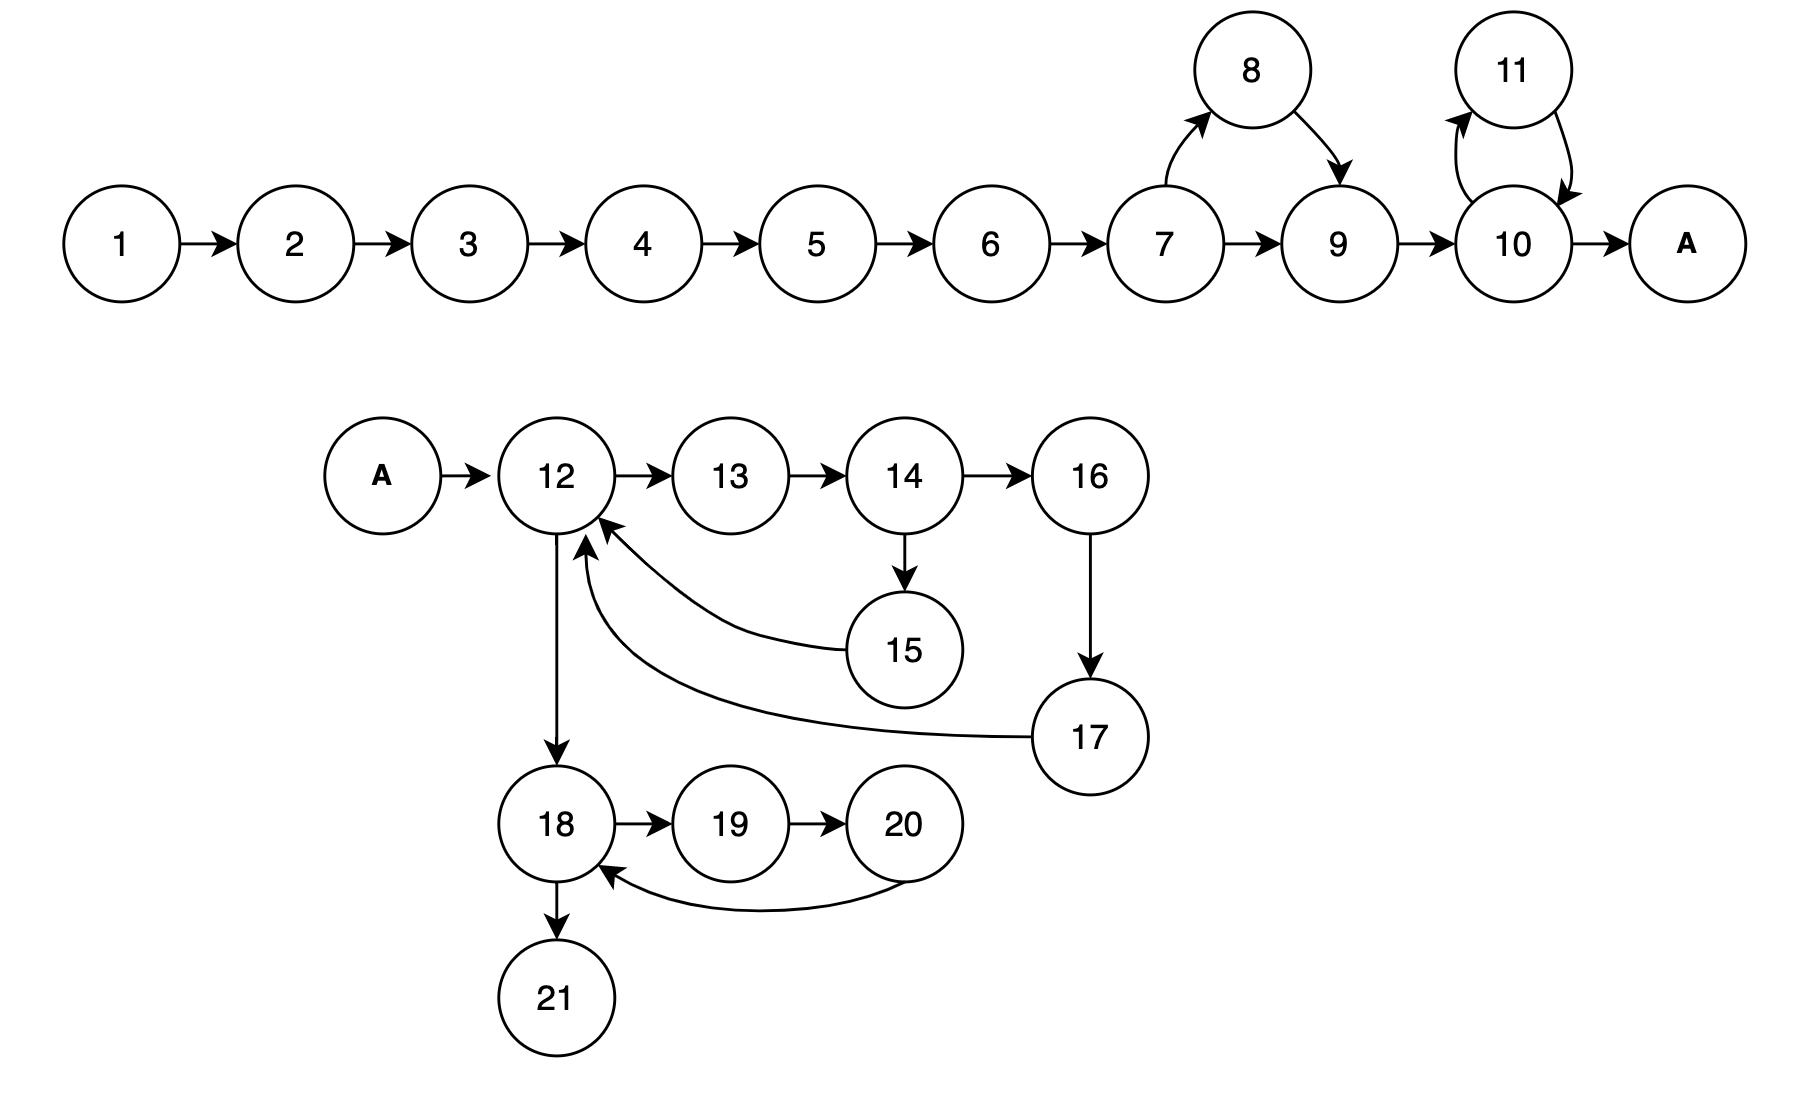
\includegraphics[width=0.9\linewidth]{inc/img/гу.png}
	\caption{Граф управления}
	\label{fig:og}
\end{figure}

\clearpage


\subsection{Информационный граф программы}

На рисунке \ref{fig:ig} представлен информационный граф программы

\begin{figure}[h!]
	\centering
	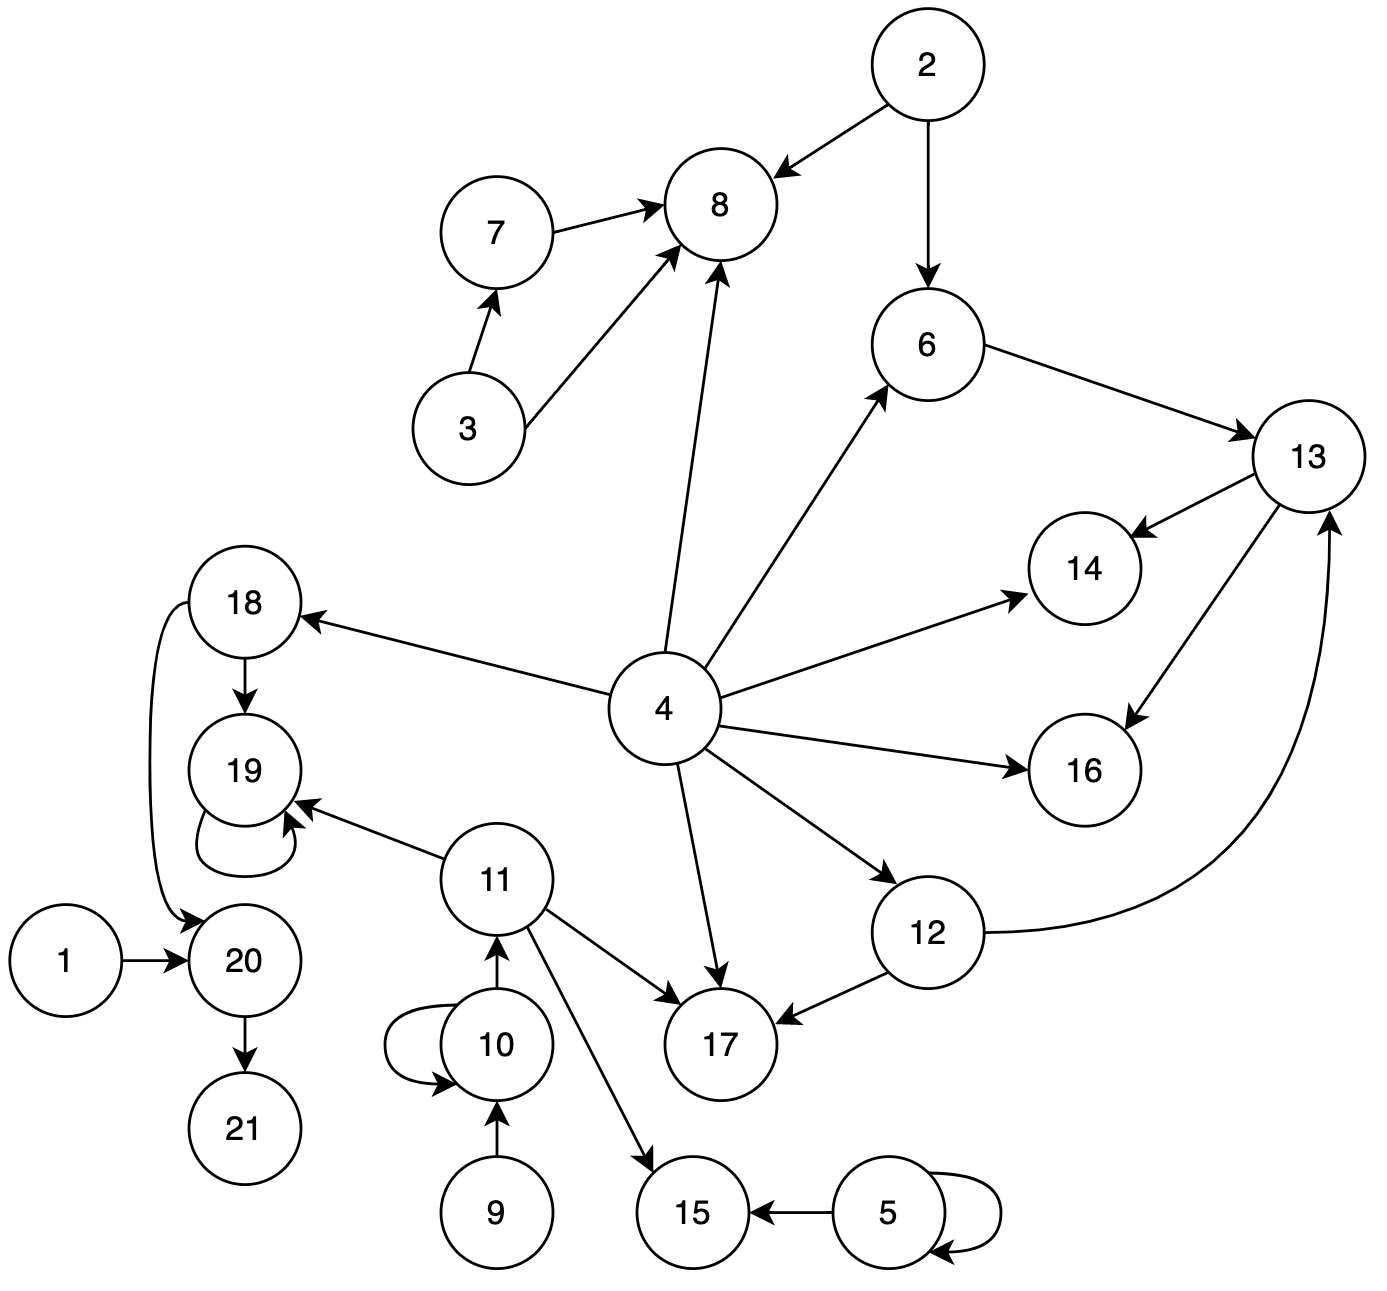
\includegraphics[width=0.9\linewidth]{inc/img/иг.png}
	\caption{Информационный граф}
	\label{fig:ig}
\end{figure}

\clearpage

\subsection{Операционная история программы}

На рисунке \ref{fig:oi} представлена операционная история программы.

\begin{figure}[h!]
	\centering
	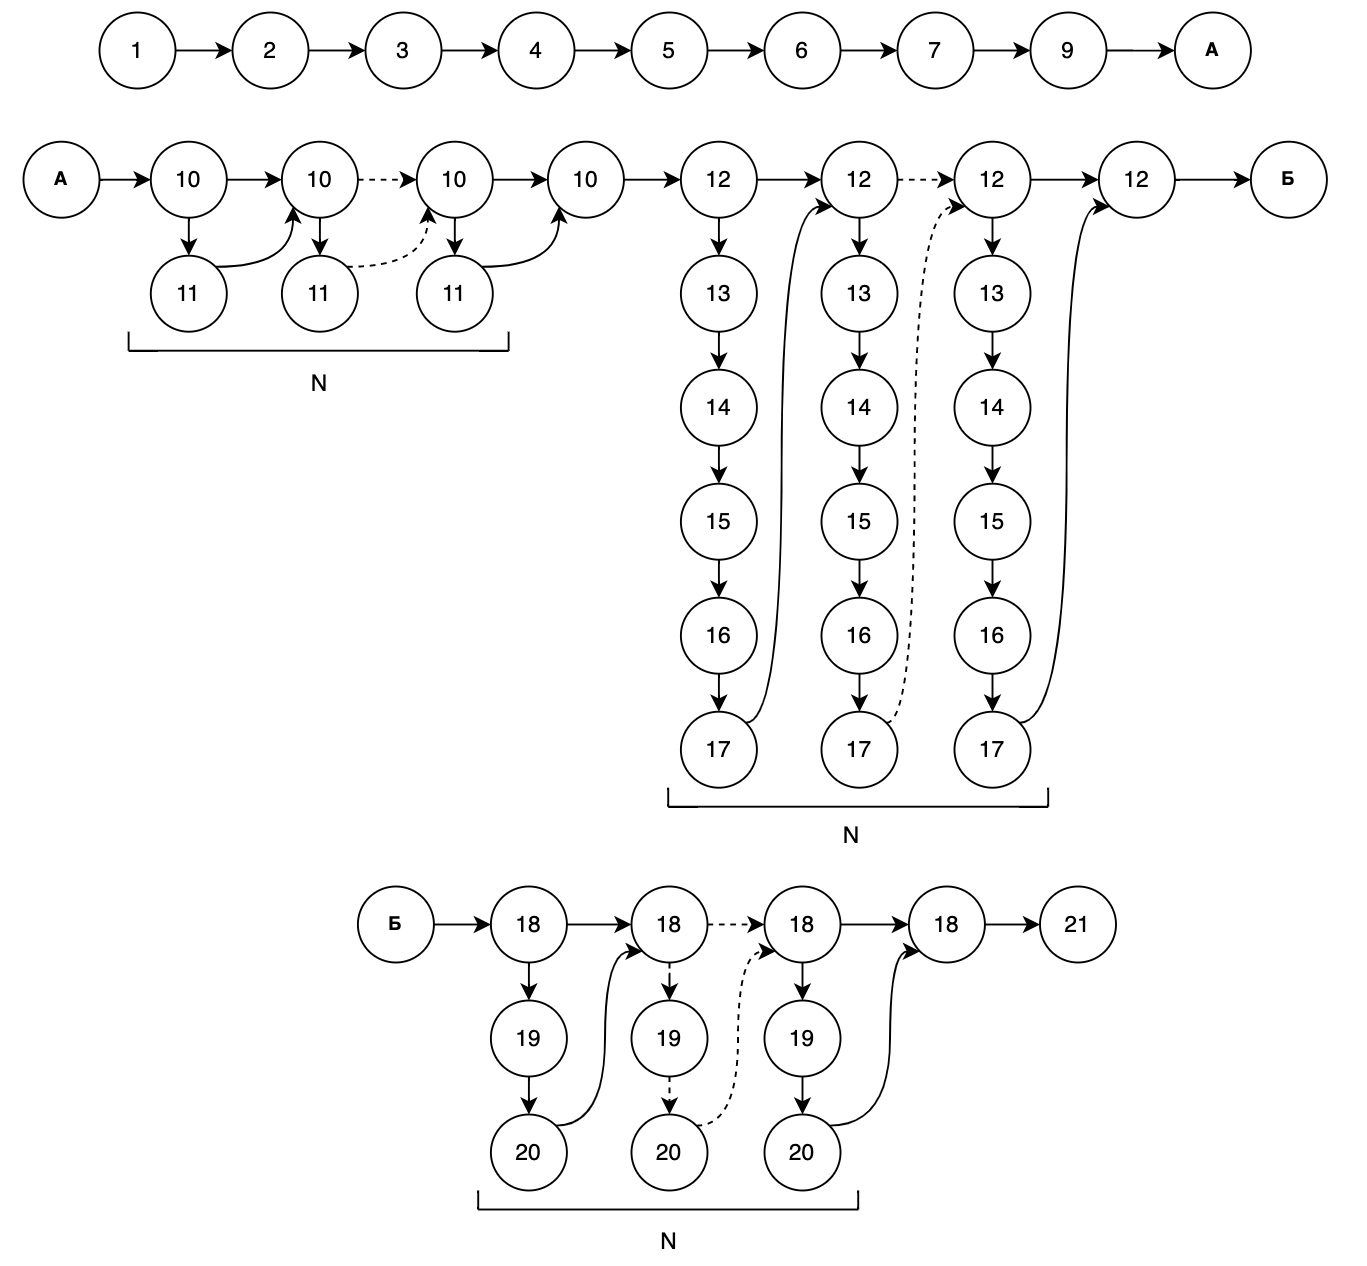
\includegraphics[width=0.9\linewidth]{inc/img/ои.png}
	\caption{Операционная история}
	\label{fig:oi}
\end{figure}

\clearpage

\subsection{Информационная история программы}

На рисунке \ref{fig:ii} представлена информационная история программы.

\begin{figure}[h!]
	\centering
	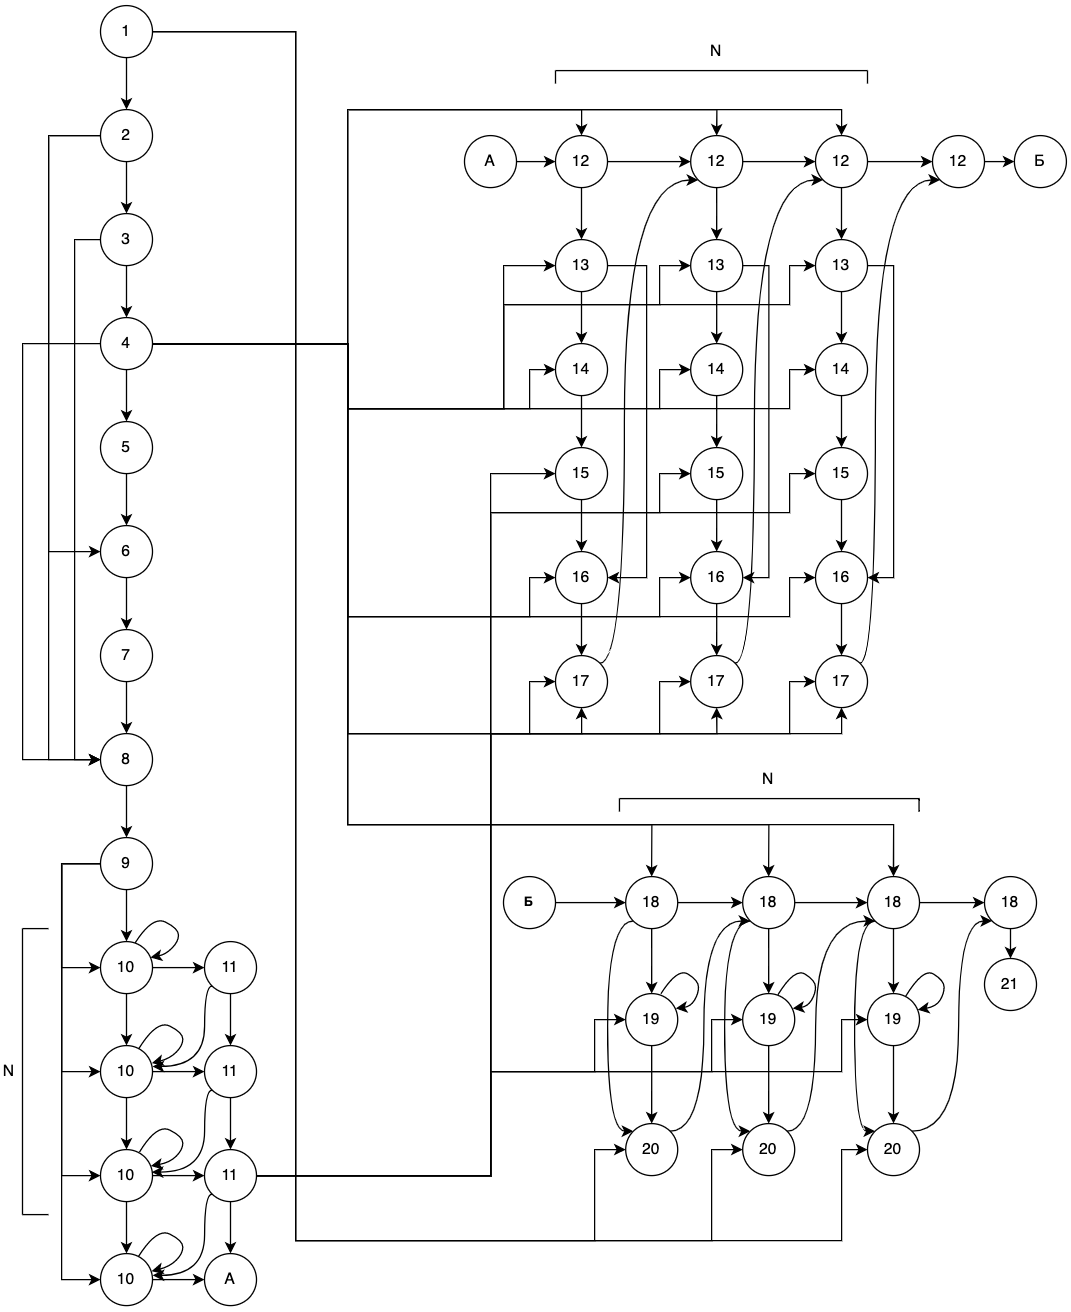
\includegraphics[width=0.9\linewidth]{inc/img/ии.png}
	\caption{Информационная история}
	\label{fig:ii}
\end{figure}

\clearpage


